\documentclass[12pt,fleqn]{article}\usepackage{../common}
\begin{document}
Ders 21

Evristirme (convolution) teknigi, iki fonksiyon uzerinde islem yaparak
ucuncu bir fonksiyon elde eder, ve ozel bir isareti vardir.

\[ f(t) * g(t) \]

Elde edilen fonksiyon $f(t)$'ye neredeyse hic benzemeyecektir. Evristirme
islemini faydali hale getiren iki sebep var. Birinci fayda formel tanimiyla
alakali. Diyelim ki ustteki iki fonksiyonun ayri ayri Laplace Transformu 

\[ F(s) = \int_0^{\infty} e^{-st} f(t) \ dt \]

\[ G(s) = \int_0^{\infty} e^{-st} g(t) \ dt \]

Iki fonksiyonun carpiminin Laplace transformunu elde etmek icin
fonksiyonlarin ayri ayri transformunu bir sekilde bir sekilde kullanan bir
formul olsa iyi olmaz miydi? Boyle bir fonksiyon var midir?

Dolayli yoldan evet. Transformlarin carpimi, fonksiyonlarin carpiminin
degil ama ``evrisimlerinin'' transformuna esittir. Yani

\[ F(s)G(s) =  \int_0^{\infty} e^{-st} (f*g)\ dt 
\ \ \ \label{1}
\]

Peki niye boyle bir kisayolun olmasi iyi bir sey? Faydayi belirttik ama
sebebini belirtmedik. 

Bunu anlamak icin once ustel serilere bakalim. Hatirlayalim, Laplace
transformunun ustel serilere (power series) paralelligi vardi

\[ F(x) = \sum a_n x^n \]

$n$'yi $t$ yapip surekli ortama gecince Laplace transformunu elde
ediyorduk.

Simdi ikinci fonksiyon

\[ G(x) = \sum b_n x^n \]

Ustteki formullerde katsayi icin $a_nb_n$ kullansam, bu $F(x)$ ve $G(x)$
ile bir sekilde baglanti yaratir miydi? Cevap dolayli yoldan
evet. Asagidaki formulde $c_n$'i $a_n,b_n$ ile ilintilendiren bir formul
lazim bize. 

\[ F(x)G(x) = \sum c_n x^n \]

Bu formul odeviniz olsun, ama bu formulu bir kere bulunca surekli ortam
icin birazdan verecegimiz formule ne kadar benzedigini goreceksiniz. 

\[ f(t)*g(t) = \int_0^t f(u)g(t-u) du \]

Ne bicim bir formul bu? Onu anlamanin en iyi yolu onu kullanarak bir seyler
hesaplamak herhalde. Not: Kabaca bir tanim soyle olabilir belki, $t$ bazli
iki fonksiyon aliniyor, sifirdan ile $t$ degeri arasindaki tum degerler $f$
icin oldugu gibi, $g$ icin tam tersi sekilde $f,g$'ye hesaplattirilip
birbirleri ile carpiliyor.

Bu arada evristirme sirabagimsiz (commutative) bir islemdir, yani 

\[ f*g = g*f \]

Evristirme formulune bakinca sirabagimsizlik bariz degil, cunku formul simetrik
durmuyor, ama evristirme formulunu (1)'deki gibi gorursek, o zaman bariz
oluyor. 

\[ \mathcal{L} (f*g) \leadsto F(s)G(s) \]

ise, $F(s)$ ve $G(s)$ carpimi sirabagimsizdir, o zaman evristirme de
sirabagimsizdir. 

Ornek

$t^2 * t$'yi hesaplayalim

\[ t^2 * t =
\int_0^t u^2 \cdot (t - u)du
\]

\[ = \frac{u^3}{3}t - \frac{u^4}{4} \bigg]_{0}^{t} = 
\frac{t^4}{3} - \frac{t^4}{4} =
\frac{t^4}{12}
\]

Pur formul kullanan cozum boyle. Ama hile (!) yaparak Laplace transformunu
kullanabiliriz. 

\[ t^2 \leadsto \frac{2}{s^3}, t \leadsto \frac{1}{s^2} \]

Bu transformlarin carpimini alirsak 

\[F(s)G(s) = \frac{2}{s^5} \]


Usttekinin ters Laplace'i nedir? 

\[ \mathcal{L}^{-1}(\frac{2}{s^5}) = \frac{1}{12}t^4 \]

Bunu nasil hemen bulduk? Bildigimiz bir ters transform soyle

\[ \mathcal{L}^{-1}(\frac{4!}{s^5}) = t^4 \]

Bunu alip iki usttekine cevirmek icin 12 ile bolmek gerekiyordu. 

Ornek

\[ f(t) * 1 = \int_0^t f(u) \ 1 \ du \]

\[  = \int_0^t f(u) du \]


Simdi evristirme isleminin Laplace Transformu ile baglantisini ispatlayacagiz. 

\[ F(s)G(s) = \int_0^{\infty}  e^{-su}f(u) du\cdot  
\int_0^{\infty}  e^{-sv} g(v) dv
\]

Usttekini cebirsel olarak bir yere ``dogru'' manipule etmeden once, belki
sunu dusunsek daha iyi olur. ``Neyi'' manipule edersek ustteki forma
geliriz? Cift entegrallerde entegre edilenleri her biri ``tek bir seyin''
fonksiyonu olan ayri gruplarin carpimi olarak gormek ise yarar, cunku o
zaman mesela ic entegral her neyse o degiskene gore digeri sabit sayilir,
disari atilabilir, vs. Yani usttekine alttaki formulden gelebiliriz

\[ = \int_{0}^{\infty} \int_{0}^{\infty} e^{-s(u+v)} f(u)g(v) du dv \]

Daha da basitlestirelim. Eger $t=u+v$ olsaydi (ki $t$ burada yeni bir
degisken olarak disaridan formule dahil ediliyor) isimiz
kolaylasirdi. $u=u$ olarak aliriz, $v$ artik kullanilmaz, $t-u = v$
yeterli.  

\[ = \int \int  e^{-st} f(u)g((t-u)) \ du \ \_\_ \ dt \]

Ustte $dt$ kullanmak istiyorum ama bu degisimi dikkatli yapmak lazim, bos
birakilan yere ne gelecegini bulmak icin Jacobian matrisini kullanmam
lazim.

\[ dudv = \frac{\partial(u,v)}{\partial(u,t)}dudt \]

\[ u = u \]

\[ v = t - u \]

\[ J = \left|\begin{array}{rr}
1 & 0 \\ -1 &1
\end{array}\right| = 1
\]

Yani 

\[ dudv = 1 \ dudt \]

O zaman 


\[ = \int \int e^{-st} f(u)g((t-u)) \ du \ dt \]

Tamam. Bir adim daha kaldi, entegral sinirlarini da degistirmek lazim. Bu
biraz daha zor olabilir. 

Ic entegrale bakalim, $u$ degisiyor, $t$ sabit tutuluyor. Daha dogrusu
$t=u+v$ olduguna gore $u+v$ bir sabit. Bir $u,v$ grafigi dusunursek, 

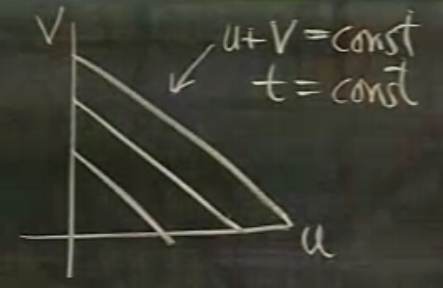
\includegraphics[height=3cm]{21_1.png}

$u+v$ gosterilen duz cizgiler uzerinde sabittir. 

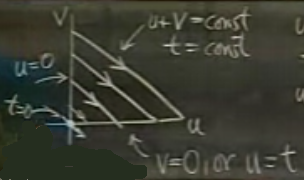
\includegraphics[height=3cm]{21_2.png}

$u$ ustteki oklar yonunde artar. Peki $u$ bolgeye soldan girdiginde degeri
nedir? Sifir. Alttan cikarken degeri nedir? O noktada $v=0$ olduguna gore,
$u+v = t$ olduguna gore, $u=t$. 

\[ = \int \int_0^t e^{-st} f(u)g((t-u)) \ du \ dt \]

Dis entegral, orijin noktasindaki $t=0$'dan baslayarak tum cizgiler icin bu
islemi yapmak istiyorum, bu islem sonsuza kadar devam ediyor. 

\[ = \int_0^{\infty} \int_0^t e^{-st} f(u)g((t-u)) \ du \ dt \]

Ispat tamamlandi. 

Laplace Transformunu ile evristirme islemi arasindaki baglantiyi gorduk. 

* * *

Evristirme cok onemli bir islemdir, ama onu kullanan pek cok kisi onu Laplace
Transformuyla alakali olarak kullanmaz. Onu oldugu gibi tek basina
kullanirlar. Bir ornek vereyim: benim kizim bir doga / cevre muhendisi
(environmental engineer), ve musterileri icin risk analizi yapmak gibi
isleri var. Bir gun bir musterisi icin, bir bilimsel makale okuyordu,
makale asit yagmuru ile alakaliydi, yagmur gelirse cevre ne kadar zarar
gorur gibi konularla ilgiliydi. Verilen zararin hesabi icin evristirme
kullaniliyor dedi, bana sordu ``bu da ne boyle?''. Makaleyi ben de okudum,
hakikaten ilgincti, yani bu alanda evristirme hesabinin olmasi ilgincti.

Sonralari diger insanlar da benzer sorularla bana geldiler. Kuzey Kutbu'nda
delme islemi yapan bir muhendis geldi mesela, delme sirasinda algilanan
radyoaktiviteyi kullanip milyonlarca yil onceki iklim sartlari hakkinda
hesap yapmakla ilgileniyordu, o da evristirme hesabini kullandi. 

O yuzden simdi ben de size pek cok alana adapte edilebilecek, genel, basit
bir model gosterecegim, bu modeli ornek olarak aklinizda tutmaniz evristirme
hesabini anlamaniz icin iyi olur. Problem radyoaktif atiklarla alakali. 

Bir fabrika radyoaktif atik uretiyor. 

$f(t)$: atim hizi (rate), $t$ sene. Iki zaman noktasini dusunursek,
$t_i,t_{i+1}$ arasinda uretilen radyoaktif atik $\approx f(t_i) \cdot
\Delta t$. Zaman araligi
kuculdukce bu hesap kesinlesecek. 

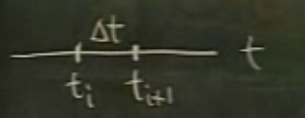
\includegraphics[height=2cm]{21_3.png}

Problemim, $t=0$'dan baslarsam $t$ aninda ne kadar radyoaktif atik
biriktiginin hesabi. Bu hesabi zorlastiran radyoaktif maddelerin ayni anda
curuyor olmasidir.

Yani bir yandan atik uretiliyor, bir yandan bu atiklar bir sekilde
radyoaktif ozelliklerini kaybediyorlar. O zaman yaptigimiz hesap uretilen
madde obeklerinin, parcalarinin birikintide ``ne kadar bekledigini'' de
hesaba katmali \textbf{ki} onun ��r�mesini de bir yandan hesaplayabilelim.

��r�me hesabi basit bir diferansiyel denklem, $t$ aninda kalan madde icin,
eger $A_0$ ile baslanirsa cozumu

\[ A_0e^{-kt} \]

$t$ ekseninin ismini degistirip $u$ yapalim (bunu niye yaptigimiz birazdan
belli olacak)

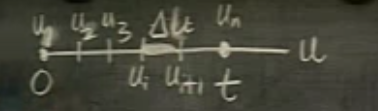
\includegraphics[height=2cm]{21_4.png}

O zaman daha once hesapladigimiz gibi $[u_i,u_{i+1}]$ arasinda uretilen
radyoaktif atik $\approx f(u_i)\Delta u$. 

$t$ aninda c�r�me ise 

\[  \approx f(u_i)\Delta u \cdot e^{-k ( \ \ \ )}\]

$e$'nin solundaki kisim atilan, eklenen kisim. ��r�me hesabina gore orasi
bir nevi $A_0$. Peki $e$'nin ustundeki bosluga ne yazilmali? Oraya eklenen
kismin curudugu zaman araligi konulmali. O zaman araligi nedir? $u_i$'da
atilmis, $t$ anina bakiyorum, o zaman $t-u_i$ araligi kadar ��r�m��
demektir. 

\[  \approx f(u_i)\Delta u \cdot e^{-k ( t-u_i )}\]

Simdi tum $u$ araliklarini alip birbiriyle toplarsam, $t$ anindaki toplami
bulurum,  

\[ \approx \sum_{i=1}^{n} f(u_i) e^{-k(t-u_i)} \Delta u \]

$\Delta u \to 0$ iken ustteki ``Riemann toplami'' suna yaklasir (araliklar
$u_1 = 0$, ve $u_n = t$ arasinda)

\[ \to \int_0^{t} f(u) e^{k(t-u)}du \]

Ustteki fonksiyon bir evrismedir, 

\[ = f(t) * e^{-kt} \]

Yani hesap at�k fonksiyonu ile ��r�me fonksiyonun bir evrismesidir
(convolution of). 

Pek cok diger problem ustteki probleme indirgenebilir, onun merceginden
anlasilablir. Mesela cop atiklarini dusunelim, ama cop atiklari ��r�m�yor
olsunlar. O zaman evristirme hesabi

\[ f(t) * 1 \]

1 kullanildi cunku ��r�me yok. 

Bir diger ornek, tavuk yetistiriliyor, 

$f(t)$ yeni tavuklarin uretilme orani (kg)

$t$ dogduklari anda civcivlerin buyume buyume orani

$t$ aninda kac kilo tavuk oldugu $f(t) * t$. 












\end{document}
